
\section{Examples Using Two Triangles}
\label{sec:example:twotri3}

PyLith features discussed in this example:
\begin{itemize}
\item Quasi-static solution
\item Mesh ASCII format
\item Dirichlet boundary conditions
\item Kinematic fault interface conditions
\item Plane strain linearly elastic material
\item VTK output
\item Linear triangular cells
\item SimpleDB spatial database
\item ZeroDispDB spatial database
\end{itemize}
All of the files necessary to run the examples are contained in the
directory \filename{examples/twocells/twotri3.}


\subsection{Overview}

This example is the simplest 2D example of a quasi-static finite
element problem (a simpler problem would consist of a 1D bar). It
is a mesh composed of two linear triangles subject to displacement
boundary conditions, assuming plane-strain linear elastic behavior.
Due to the simple geometry of the problem, the mesh may be constructed
by hand, using PyLith mesh ASCII format. In this example, we will
walk through the steps necessary to construct, run, and view three
problems that use the same mesh. In addition to this manual, each
of the files for the example problem includes extensive comments.


\subsection{Mesh Description}

The mesh consists of two triangles forming a square with edge lengths
of one unit (Figure \vref{fig:twotri3-mesh}). The mesh geometry and
topology are described in the file \filename{twotri3.mesh}, which is
in PyLith mesh ASCII format. This file format is described in Appendix
\vref{cha:formats}. This file describes the dimensionality of
the problem (1D, 2D, or 3D), the coordinates of the vertices (nodes),
the vertices composing each cell (element), the material ID to be
associated with each cell, and groups of vertices that may be used
to define faults or surfaces to which boundary conditions may be applied.

\begin{figure}
  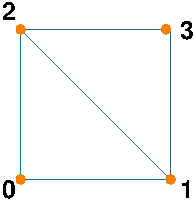
\includegraphics{examples/figs/twotri3-mesh}
  \caption{Mesh composed of two linear triangular cells used in the
    example problems.}
  \label{fig:twotri3-mesh}
\end{figure}


\subsection{Additional Common Information}

In addition to the mesh, the three example problems share additional
information. For problems of this type, it is generally useful to
create a file named \filename{pylithapp.cfg} in the working directory,
since this file is read automatically every time PyLith is
run. Settings specific to a particular problem may be placed in other
\filename{cfg} files, as described later, and then those files are
placed on the command line. The settings contained in
\filename{pylithapp.cfg} for this problem consist of:
\begin{inventory}
  \facilityitem{pylithapp.journal.info}{Settings that control the verbosity of
    the output for the different components.}
  \facilityitem{pylithapp.mesh\_generator}{Settings that control mesh importing,
    such as the importer type, the filename, and the spatial dimension
    of the mesh.}
  \facilityitem{pylithapp.timedependent}{Settings that control the problem, such
    as the total time, time step size, and spatial dimension.}
  \facilityitem{pylithapp.timedependent.materials}{Settings that control the material
    type, specify which material IDs are to be associated with a particular
    material type, and give the name of the spatial database containing
    the physical  properties for the material. The quadrature information
    is also given.}
  \facilityitem{pylithapp.petsc}{PETSc settings to use for the problem, such as
    the preconditioner type.}
\end{inventory}
All of the problems in this directory use the same material database,
as specified under \object{pylithapp.timedependent.materials} in
\filename{pylithapp.cfg}. This information is contained in the file
\filename{matprops.spatialdb}. Although the material model is
specified in \filename{pylithapp.cfg}, the values for the physical
properties of the material are given in
\filename{matprops.spatialdb}. For this example, values describing
elastic plane strain material properties are given at a single point,
resulting in uniform material properties.


\subsection{Axial Displacement Example}

The first example problem is extension of the mesh along the diagonal
extending from the lower left to the upper right of the square mesh.
Parameter settings that augment those in \filename{pylithapp.cfg} are
contained in the file \filename{axialdisp.cfg}. These settings are:
\begin{inventory}
  \facilityitem{pylithapp.timedependent}{Specifies an implicit formulation for
    the problem and specifies the array of boundary conditions.}
  \facilityitem{pylithapp.timedependent.bc.bc}{Defines which degrees of freedom
    are being constrained (x and y), gives the label (defined in \filename{twotri3.mesh})
    defining the points desired, assigns a label to the boundary condition
    set, and gives the name of the spatial database with the values for
    the Dirichlet boundary condition (\filename{axialdisp.spatialdb}).}
  \facilityitem{pylithapp.problem.formulation.output.output.writer}{Gives the
    base filename for VTK output (\filename{axialdisp.vtk}).}
  \facilityitem{pylithapp.timedependent.materials.material.output}{Gives the base
    filename for state variable output files (\filename{axialdisp-statevars.vtk}).}
\end{inventory}
The values for the Dirichlet boundary condition are given in the file
\filename{axialdisp.spatialdb}, as specified in
\filename{axialdisp.cfg}.  The format of all spatial database files is
similar. In this case, the desired displacement values are given at
two points (lower left and upper right). Since data are being
specified at points (rather than being uniform over the mesh, for
example), the data dimension is one.

The files containing common information (\filename{twotri3.mesh},
\filename{pylithapp.cfg}, \filename{matprops.spatialdb}) along with
the problem-specific files (\filename{axialdisp.cfg},
\filename{axialdisp.spatialdb}) provide a complete description of the
problem, and we can then run this example by typing
\begin{shell}
$ pylith axialdisp.cfg
\end{shell}
Once the problem has run, three files will be produced. The first
file is named \filename{axialdisp\_t0000000.vtk}. The \filename{t0000000}
indicates that the output is for the first (and only) time step, corresponding
to an elastic solution. This file contains mesh information as well
as displacement values at the mesh vertices. The second file is named
\filename{axialdisp-statevars\_t0000000.vtk}. This file contains the
state variables for each cell. The default fields are the total strain
and stress fields. Since the cells are linear triangles, there is
a single quadrature point for each cell and thus a single set of stress
and strain values for each cell. The final file (\filename{axialdisp-statevars\_info.vtk})
gives the material properties used for the problem. Since we have
not specified which properties to write, the default properties (\texttt{mu},
\texttt{lambda}, \texttt{density}) are written. All of the \filename{vtk}
files may be used with a number of visualization packages. If the
problem ran correctly, you should be able to generate a figure such
as Figure \vref{fig:twotri3-axial}, which was generated using ParaView.

\begin{figure}
  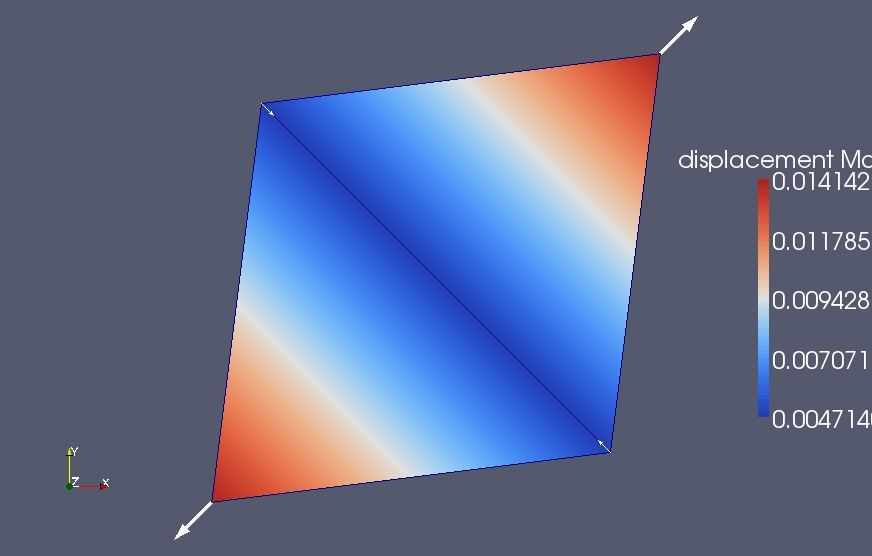
\includegraphics[scale=0.33]{examples/figs/twotri3-axialdisp}
  \caption{Color contours and vectors of displacement for the axial
    displacement example using a mesh composed of two linear triangular
    cells.}
  \label{fig:twotri3-axial}
\end{figure}


\subsection{Shear Displacement Example}

The next example problem is shearing of the mesh in the y direction
using displacements applied along the positive and negative x boundaries.
Parameter settings that augment those in \filename{pylithapp.cfg} are
contained in the file \filename{sheardisp.cfg}. These settings include:
\begin{inventory}
  \facilityitem{pylithapp.timedependent.bc.x\_neg}{Specifies the boundary conditions
    for the left side of the mesh, defining which degrees of freedom are
    being constrained (x and y), giving the label (\facility{x\_neg}, defined
    in \filename{twotri3.mesh}) defining the points desired, assigning a
    label to the boundary condition set, and giving the name of the spatial
    database with the values for the Dirichlet boundary condition (\filename{sheardisp.spatialdb}).}
  \facilityitem{pylithapp.timedependent.bc.x\_pos}{Specifies the boundary conditions
    for the left side of the mesh, defining which degrees of freedom are
    being constrained (y only), giving the label (\facility{x\_pos}, defined
    in \filename{twotri3.mesh}) defining the points desired, assigning a
    label to the boundary condition set, and giving the name of the spatial
    database with the values for the Dirichlet boundary condition (\filename{sheardisp.spatialdb}).}
\end{inventory}
The files containing common information (\filename{twotri3.mesh},
\filename{pylithapp.cfg}, \filename{matprops.spatialdb}) along with
the problem-specific files (\filename{sheardisp.cfg},
\filename{sheardisp.spatialdb}) provide a complete description of the
problem, and we can then run this example by typing
\begin{shell}
$ pylith sheardisp.cfg
\end{shell}
Once the problem has run, three files will be produced as in the
previous example. If the problem ran correctly, you should be able to
generate a figure such as Figure \vref{fig:twotri-shear}, which was
generated using ParaView.

\begin{figure}
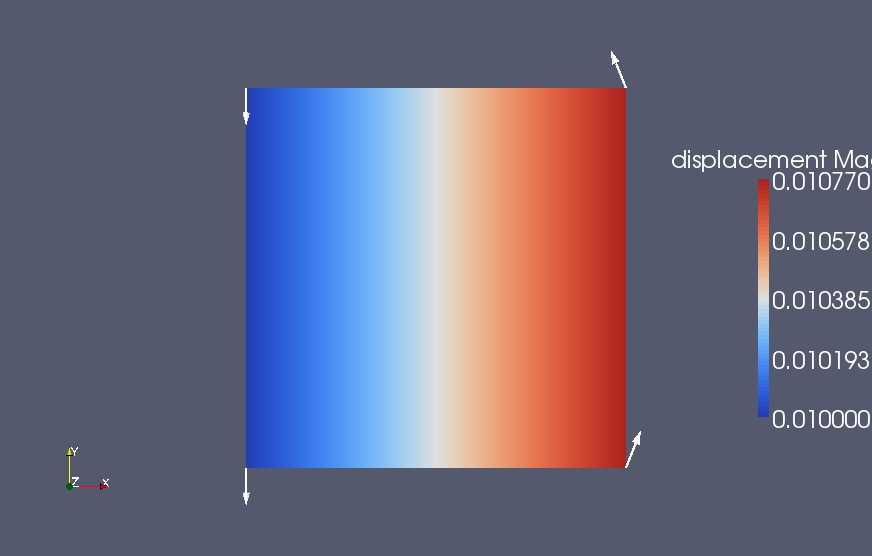
\includegraphics[scale=0.33]{examples/figs/twotri3-sheardisp}
\caption{Color contours and vectors of displacement for the shear
  displacement example using a mesh composed of two linear triangular
  cells.}
\label{fig:twotri-shear}
\end{figure}


\subsection{Kinematic Fault Slip Example}

The next example problem is left-lateral fault slip applied between
the two triangular cells using kinematic cohesive cells. The lower
left and upper right boundaries are held fixed in the x and y directions.
Parameter settings that augment those in \filename{pylithapp.cfg} are
contained in the file \filename{dislocation.cfg}. The solution corresponds
to rigid body rotation of each triangular cell. As a result, the tractions
on the fault are zero. These settings include:
\begin{inventory}
  \facilityitem{pylithapp.journal.info}{Turns on journaling for 1D quadrature
    (used for 2D faults) and for cohesive kinematic faults.}
  \facilityitem{pylithapp.timedependent.bc.bc}{Defines which degrees of freedom
    are being constrained (x and y), gives the label (defined in \filename{twotri3.mesh})
    defining the points desired, and assigns a label to the boundary condition
    set. In this case, rather than specifying a spatial database file
    with the values for the Dirichlet boundary condition, the default
    database (ZeroDispDB) for Dirichlet boundary conditions is used, which
    sets the displacements to zero.}
  \facilityitem{pylithapp.timedependent.interfaces}{Gives the label (defined in
    \filename{twotri3.mesh}) defining the points on the fault, provides
    quadrature information, and then gives database names for material
    properties (needed for conditioning), fault slip, peak fault slip
    rate, and fault slip time.}
  \facilityitem{pylithapp.timedependent.interfaces.fault.output.writer}{Gives
    the base filename for cohesive cell output files (\filename{dislocation-fault.vtk}).}
\end{inventory}
Rather than specifying the displacement boundary conditions in a
spatial database file, we use the default behavior for Dirichlet
boundary conditions, which is a uniform, constant displacement of
zero.

The fault example requires three additional database files that were
not needed for the simple displacement examples. The first file
(\filename{dislocation\_slip.spatialdb}) specifies 0.01 m of
left-lateral fault slip for the entire fault.  The data dimension is
zero since the same data are applied to all points in the set. The
default slip time function is a step-function, so we also must provide
the time at which slip begins. The elastic solution is associated with
advancing from $t=-dt$ to $t=0$, so we set the slip initiation time
for the step-function to 0 in
\filename{dislocation\_sliptime.spatialdb}.

The files containing common information (\filename{twotri3.mesh},
\filename{pylithapp.cfg}, \filename{matprops.spatialdb}) along with
the problem-specific files (\filename{dislocation.cfg},
\filename{dislocation\_slip.spatialdb},
\filename{dislocation\_sliptime.spatialdb}) provide a complete
description of the problem, and we can then run this example by typing
\begin{shell}
$ pylith dislocation.cfg
\end{shell}
Once the problem has run, five files are produced. In addition to the
files produced in the previous two examples, this example produces two
files associated with the fault interface. The file
\filename{dislocation-fault\_t0000000.vtk} gives the fault slip for
each vertex on the fault along with the computed traction change for
the cohesive cell. The file \filename{dislocation-fault\_info.vtk}
provides information such as the normal direction, final slip, and
slip time for each vertex on the fault. If the problem ran correctly,
you should be able to generate a figure such as Figure
\vref{fig:twotri-disloc}, which was generated using ParaView.

\begin{figure}
  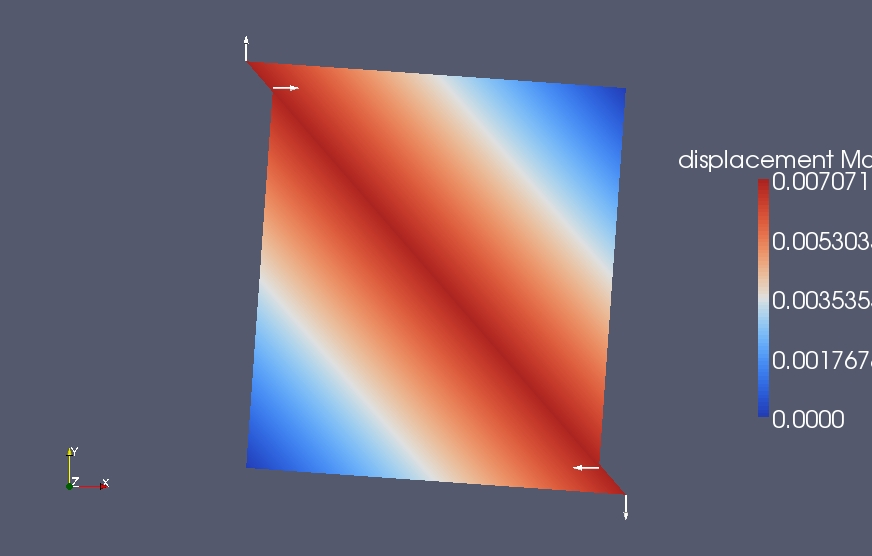
\includegraphics[scale=0.33]{examples/figs/twotri3-dislocation}
  \caption{Color contours and vectors of displacement for the kinematic fault
    example using a mesh composed of two linear triangular cells.}
  \label{fig:twotri-disloc}
\end{figure}

% End of file
